\documentclass[11pt]{article}
\usepackage[margin=0.8in]{geometry}
\usepackage{amsmath}
\usepackage{amssymb}
\usepackage{amsthm}
\usepackage{enumitem}
\usepackage{xcolor}
\usepackage{tcolorbox}
\usepackage{tikz}
\usetikzlibrary{shapes.geometric, arrows, positioning}

\title{Rigorous Guide to Testing Independence\\ORF 309}
\author{}
\date{}

\newtheorem{definition}{Definition}
\newtheorem{theorem}{Theorem}
\newtheorem{example}{Example}

\tikzstyle{startstop} = [rectangle, rounded corners, minimum width=3cm, minimum height=1cm,text centered, draw=black, fill=red!30]
\tikzstyle{process} = [rectangle, minimum width=3cm, minimum height=1cm, text centered, draw=black, fill=orange!30]
\tikzstyle{decision} = [diamond, minimum width=3cm, minimum height=1cm, text centered, draw=black, fill=green!30, aspect=2]
\tikzstyle{arrow} = [thick,->,>=stealth]

\begin{document}

\maketitle

\section{Fundamental Definitions}

\begin{definition}[Independence of Two Events]
Events $A$ and $B$ are \textbf{independent}, denoted $A \perp B$, if and only if:
\begin{equation}
\boxed{P(A \cap B) = P(A) \cdot P(B)}
\end{equation}
\end{definition}

\begin{definition}[Independence of Random Variables]
Random variables $X$ and $Y$ are \textbf{independent}, denoted $X \perp Y$, if and only if:

\textbf{Discrete case:}
\begin{equation}
P(X = x, Y = y) = P(X = x) \cdot P(Y = y) \quad \text{for all } x, y
\end{equation}

\textbf{Continuous case:}
\begin{equation}
f_{X,Y}(x, y) = f_X(x) \cdot f_Y(y) \quad \text{for all } x, y
\end{equation}
\end{definition}

\begin{tcolorbox}[colback=red!5!white,colframe=red!75!black,title=CRITICAL DISTINCTION]
\textbf{Independent} $\neq$ \textbf{Mutually Exclusive}

If $A \cap B = \emptyset$ and $P(A), P(B) > 0$, then $A$ and $B$ are \textbf{DEPENDENT}.

\textbf{Why?} Because:
\begin{align*}
P(A \cap B) &= 0 \quad \text{(mutually exclusive)}\\
P(A) \cdot P(B) &> 0 \quad \text{(both positive)}\\
\Rightarrow P(A \cap B) &\neq P(A) \cdot P(B)
\end{align*}
\end{tcolorbox}

\section{Equivalent Conditions for Independence}

\begin{theorem}[Equivalent Conditions for Independence of Events]
If $P(A) > 0$ and $P(B) > 0$, the following are equivalent:
\begin{enumerate}
    \item $P(A \cap B) = P(A) \cdot P(B)$ \quad \textbf{(Definition)}

    \item $P(A | B) = P(A)$ \quad \textbf{(B doesn't affect A)}

    \item $P(B | A) = P(B)$ \quad \textbf{(A doesn't affect B)}

    \item $P(A | B) = P(A | B^c)$ \quad \textbf{(A's probability unchanged by B)}

    \item $P(B | A) = P(B | A^c)$ \quad \textbf{(B's probability unchanged by A)}
\end{enumerate}
\end{theorem}

\begin{tcolorbox}[colback=blue!5!white,colframe=blue!75!black,title=Proof Strategy]
To prove independence: Show ANY one of these conditions holds.

To prove dependence: Show ANY one of these conditions FAILS.
\end{tcolorbox}

\begin{theorem}[Properties of Independence]
If $A \perp B$, then:
\begin{itemize}
    \item $A \perp B^c$
    \item $A^c \perp B$
    \item $A^c \perp B^c$
\end{itemize}
\end{theorem}

\section{Step-by-Step Testing Procedure}

\subsection{For Events A and B}

\begin{tcolorbox}[colback=yellow!10!white,colframe=orange!75!black,title=Step-by-Step Guide]
\textbf{Step 1: Identify what you know}
\begin{itemize}
    \item Do you know $P(A)$, $P(B)$, $P(A \cap B)$?
    \item Do you know conditional probabilities like $P(A|B)$ or $P(B|A)$?
\end{itemize}

\textbf{Step 2: Choose your test}

\textbf{Option A:} If you know $P(A)$, $P(B)$, and $P(A \cap B)$:
\begin{equation}
\text{Check if } P(A \cap B) \stackrel{?}{=} P(A) \cdot P(B)
\end{equation}

\textbf{Option B:} If you know $P(A|B)$ and $P(A)$:
\begin{equation}
\text{Check if } P(A|B) \stackrel{?}{=} P(A)
\end{equation}

\textbf{Option C:} If you know $P(A|B)$ and $P(A|B^c)$:
\begin{equation}
\text{Check if } P(A|B) \stackrel{?}{=} P(A|B^c)
\end{equation}

\textbf{Step 3: Make your conclusion}
\begin{itemize}
    \item If equal: Events are \textbf{independent}
    \item If not equal: Events are \textbf{dependent}
\end{itemize}
\end{tcolorbox}

\subsection{For Random Variables X and Y}

\begin{tcolorbox}[colback=green!5!white,colframe=green!75!black,title=Testing Independence of Random Variables]

\textbf{Method 1: Joint Distribution Factorization}

\textbf{Discrete:} Check if $p_{X,Y}(x, y) = p_X(x) \cdot p_Y(y)$ for ALL $(x, y)$

\textbf{Continuous:} Check if $f_{X,Y}(x, y) = f_X(x) \cdot f_Y(y)$ for ALL $(x, y)$

\textbf{Shortcut:} If the joint PMF/PDF factors as $g(x) \cdot h(y)$ (one function of $x$ only, one function of $y$ only) over a rectangular domain, then $X \perp Y$.

\vspace{0.3cm}

\textbf{Method 2: Conditional Distribution}

Check if $P(X = x | Y = y) = P(X = x)$ for all $x, y$ (discrete case)

Or equivalently: $f_{X|Y}(x|y) = f_X(x)$ for all $x, y$ (continuous case)

\vspace{0.3cm}

\textbf{Method 3: Expectation Test}

If $X \perp Y$, then $E[g(X) \cdot h(Y)] = E[g(X)] \cdot E[h(Y)]$ for any functions $g, h$.

Special case: $E[XY] = E[X] \cdot E[Y]$

\textbf{WARNING:} The converse is FALSE. $E[XY] = E[X]E[Y]$ does NOT imply independence.

\vspace{0.3cm}

\textbf{Method 4: Covariance Test}

If $X \perp Y$, then $\text{Cov}(X, Y) = 0$ (uncorrelated).

\textbf{WARNING:} The converse is FALSE. $\text{Cov}(X, Y) = 0$ does NOT imply independence.
\end{tcolorbox}

\section{Worked Examples}

\begin{example}[Problem 1c from S2025 Midterm]
\textbf{Setup:}
\begin{itemize}
    \item $P(A) = 0.8$ (prob of getting question 1 correct)
    \item $P(B|A) = 0.6$ (prob of question 2 correct given question 1 correct)
    \item $P(B|A^c) = 0.1$ (prob of question 2 correct given question 1 wrong)
\end{itemize}

\textbf{Question:} Are $A$ and $B$ independent?

\textbf{Solution:}

First, calculate $P(B)$ using LOTP:
\begin{align*}
P(B) &= P(B|A)P(A) + P(B|A^c)P(A^c)\\
&= 0.6 \times 0.8 + 0.1 \times 0.2\\
&= 0.48 + 0.02 = 0.5
\end{align*}

\textbf{Test 1:} Compare $P(B|A)$ with $P(B)$
\begin{equation}
P(B|A) = 0.6 \neq 0.5 = P(B)
\end{equation}

\textbf{Conclusion:} $A$ and $B$ are \textbf{DEPENDENT}.

\textbf{Alternative Test:} Compare $P(B|A)$ with $P(B|A^c)$
\begin{equation}
P(B|A) = 0.6 \neq 0.1 = P(B|A^c)
\end{equation}

Same conclusion: \textbf{DEPENDENT}.

\textbf{Verification using definition:}
\begin{align*}
P(A \cap B) &= P(B|A)P(A) = 0.6 \times 0.8 = 0.48\\
P(A) \cdot P(B) &= 0.8 \times 0.5 = 0.4\\
P(A \cap B) &\neq P(A) \cdot P(B)
\end{align*}

Therefore \textbf{DEPENDENT}.
\end{example}

\begin{example}[Geometric Wait Times - Problem 2 from S2025 Midterm]
\textbf{Setup:} $X$ = delay to New York (Geom(0.1)), $Y$ = delay to Trenton (Geom(0.2))

\textbf{Given:} The delays are probabilistically independent.

\textbf{Question:} Given $Y = 5$, what is $E[X | Y = 5]$?

\textbf{Solution:}

Since $X \perp Y$, conditioning on $Y$ doesn't change the distribution of $X$:
\begin{equation}
E[X | Y = 5] = E[X] = \frac{1}{0.1} = 10
\end{equation}

\textbf{Key insight:} If $X \perp Y$, then any information about $Y$ is irrelevant for $X$.
\end{example}

\begin{example}[Testing with Joint PMF]
\textbf{Setup:} Suppose $(X, Y)$ has joint PMF:
\begin{equation}
p_{X,Y}(x, y) = \frac{1}{12} \quad \text{for } (x, y) \in \{(1, 1), (1, 2), (2, 1), (2, 2)\}
\end{equation}

Wait, that doesn't sum to 1. Let me recalculate:
\begin{equation}
p_{X,Y}(x, y) = \frac{1}{4} \quad \text{for } (x, y) \in \{(1, 1), (1, 2), (2, 1), (2, 2)\}
\end{equation}

\textbf{Marginals:}
\begin{align*}
p_X(1) &= p_{X,Y}(1, 1) + p_{X,Y}(1, 2) = \frac{1}{4} + \frac{1}{4} = \frac{1}{2}\\
p_X(2) &= p_{X,Y}(2, 1) + p_{X,Y}(2, 2) = \frac{1}{4} + \frac{1}{4} = \frac{1}{2}\\
p_Y(1) &= p_{X,Y}(1, 1) + p_{X,Y}(2, 1) = \frac{1}{4} + \frac{1}{4} = \frac{1}{2}\\
p_Y(2) &= p_{X,Y}(1, 2) + p_{X,Y}(2, 2) = \frac{1}{4} + \frac{1}{4} = \frac{1}{2}
\end{align*}

\textbf{Test independence:}
\begin{align*}
p_{X,Y}(1, 1) &= \frac{1}{4}\\
p_X(1) \cdot p_Y(1) &= \frac{1}{2} \cdot \frac{1}{2} = \frac{1}{4}
\end{align*}

Check for all pairs:
\begin{itemize}
    \item $(1, 1)$: $\frac{1}{4} = \frac{1}{2} \cdot \frac{1}{2}$ \checkmark
    \item $(1, 2)$: $\frac{1}{4} = \frac{1}{2} \cdot \frac{1}{2}$ \checkmark
    \item $(2, 1)$: $\frac{1}{4} = \frac{1}{2} \cdot \frac{1}{2}$ \checkmark
    \item $(2, 2)$: $\frac{1}{4} = \frac{1}{2} \cdot \frac{1}{2}$ \checkmark
\end{itemize}

\textbf{Conclusion:} $X \perp Y$ (independent).
\end{example}

\begin{example}[A Dependent Example]
\textbf{Setup:} Roll a fair die. Let:
\begin{itemize}
    \item $A$ = event that die shows an even number
    \item $B$ = event that die shows a number greater than 4
\end{itemize}

\textbf{Calculate:}
\begin{align*}
P(A) &= P(\{2, 4, 6\}) = \frac{3}{6} = \frac{1}{2}\\
P(B) &= P(\{5, 6\}) = \frac{2}{6} = \frac{1}{3}\\
P(A \cap B) &= P(\{6\}) = \frac{1}{6}
\end{align*}

\textbf{Test:}
\begin{align*}
P(A) \cdot P(B) &= \frac{1}{2} \cdot \frac{1}{3} = \frac{1}{6}\\
P(A \cap B) &= \frac{1}{6}
\end{align*}

\textbf{Conclusion:} $A \perp B$ (independent)!

This might be surprising, but it's correct.
\end{example}

\section{Common Mistakes and Pitfalls}

\begin{tcolorbox}[colback=red!10!white,colframe=red!75!black,title=Common Mistakes]
\begin{enumerate}
    \item \textbf{Mutually exclusive $\neq$ independent}

    If $A \cap B = \emptyset$ and $P(A), P(B) > 0$, then $A$ and $B$ are dependent.

    \item \textbf{Uncorrelated $\neq$ independent}

    $\text{Cov}(X, Y) = 0$ does NOT imply $X \perp Y$.

    \item \textbf{$E[XY] = E[X]E[Y]$ $\neq$ independence}

    This is a necessary condition but NOT sufficient.

    \item \textbf{$P(A|B) + P(A|B^c) \neq 1$}

    The correct identity is: $P(A|B) + P(A^c|B) = 1$

    \item \textbf{Pairwise independence $\neq$ mutual independence}

    Events can be pairwise independent without being mutually independent.

    \item \textbf{Must check ALL values}

    For random variables, you must verify $p_{X,Y}(x, y) = p_X(x) \cdot p_Y(y)$ for ALL $(x, y)$, not just some values.

    \item \textbf{Given independence in the problem}

    If the problem states events/variables are independent, USE IT! Don't try to verify it again.
\end{enumerate}
\end{tcolorbox}

\section{Quick Reference Checklist}

\subsection{To Prove Independence}

\begin{itemize}[leftmargin=*]
    \item[\checkmark] Show $P(A \cap B) = P(A) \cdot P(B)$
    \item[\checkmark] Show $P(A|B) = P(A)$ (or $P(B|A) = P(B)$)
    \item[\checkmark] Show joint PMF/PDF factors: $p_{X,Y}(x, y) = g(x) \cdot h(y)$ over rectangular domain
    \item[\checkmark] Use given information (if problem states they're independent)
\end{itemize}

\subsection{To Prove Dependence}

\begin{itemize}[leftmargin=*]
    \item[\checkmark] Show $P(A \cap B) \neq P(A) \cdot P(B)$
    \item[\checkmark] Show $P(A|B) \neq P(A)$ (or $P(B|A) \neq P(B)$)
    \item[\checkmark] Show $P(A|B) \neq P(A|B^c)$ (or $P(B|A) \neq P(B|A^c)$)
    \item[\checkmark] Show joint PMF/PDF does NOT factor for some $(x, y)$
\end{itemize}

\subsection{Warning Signs of Dependence}

\begin{itemize}[leftmargin=*]
    \item Problem says "given that..." and it affects probabilities
    \item Conditional probability differs from marginal probability
    \item Events describe related outcomes (e.g., "both depend on understanding")
    \item Joint distribution doesn't factor
\end{itemize}

\section{Decision Tree}

\begin{center}
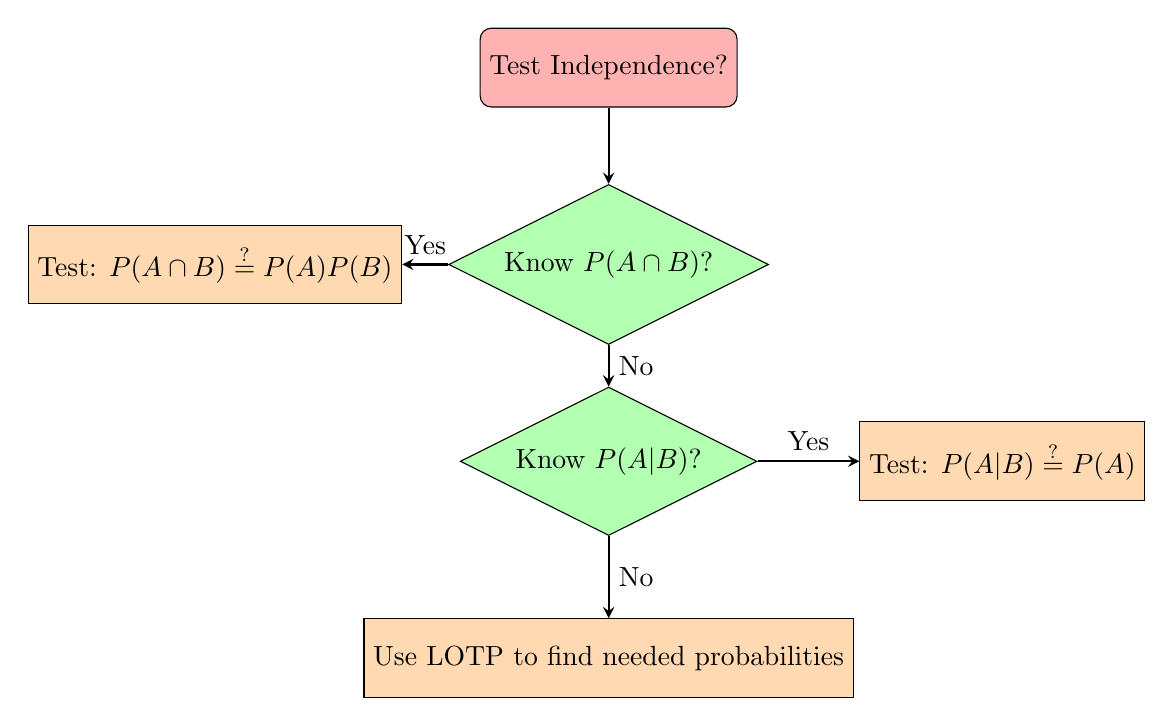
\begin{tikzpicture}[node distance=2cm]

\node (start) [startstop] {Test Independence?};
\node (check1) [decision, below of=start, yshift=-0.5cm] {Know $P(A \cap B)$?};
\node (test1) [process, left of=check1, xshift=-3cm] {Test: $P(A \cap B) \stackrel{?}{=} P(A)P(B)$};
\node (check2) [decision, below of=check1, yshift=-0.5cm] {Know $P(A|B)$?};
\node (test2) [process, right of=check2, xshift=3cm] {Test: $P(A|B) \stackrel{?}{=} P(A)$};
\node (test3) [process, below of=check2, yshift=-0.5cm] {Use LOTP to find needed probabilities};

\draw [arrow] (start) -- (check1);
\draw [arrow] (check1) -- node[anchor=south] {Yes} (test1);
\draw [arrow] (check1) -- node[anchor=west] {No} (check2);
\draw [arrow] (check2) -- node[anchor=south] {Yes} (test2);
\draw [arrow] (check2) -- node[anchor=west] {No} (test3);

\end{tikzpicture}
\end{center}

\end{document}
